\secnumbersection{MARCO CONCEPTUAL}

Para abordar nuestro problema, primero debemos definir algunos conceptos que han
sido mencionados en las secciones anteriores de forma más formal, tales como, la
web semántica, \textit{SPARQL}, \textit{RDF} y el contexto en el que estos se
utilizan. Para esto, nos apoyaremos en las siguientes definiciones.

\subsection{Web Semántica}

La red informática mundial, \textit{World Wide Web} o simplemente \textit{Web}
es el sistema de información público más importante desarrollado en los últimos
30 años, el cual permite la transmisión de documentos electrónicos identificados
por URIs \textit{(Uniform Resource Identifiers)}, los cuales pueden estar
enlazados a otros documentos a través de hipertexto y que se encuentran
disponibles utilizando servicios de la internet.

La \textit{World Wide Web} fue diseñada como un espacio para la información con
el objetivo de no solo ser útil para las comunicaciones entre humanos, sino que
también un lugar donde las máquinas podrían ayudar y participar. Sin embargo,
uno de los principales problemas de la \textit{Web} es que la mayor parte de su
contenido ha sido diseñado para ser consumido por humanos, lo que implica que
para las máquinas y el software no es fácil acceder e interpretar el contenido
disponible, incluso si este proviene de una base de datos estructurada a través
de columnas claras y tipificadas. La web semántica busca desarrollar
herramientas, lenguajes, protocolos y estándares que permitan, tanto a maquinas
como humanos, procesar toda la información disponible en la \textit{Web}. En
base a esto, podemos definir a la web semántica como la idea de generar una red
de datos en la \textit{Web}, hasta cierto punto, una base de datos global.
\cite{berners1998semantic}

\subsection{Arquitectura de la web semántica}

La web semántica está construida en base a múltiples bloques, los cuales
representan estándares y lenguajes utilizados para lograr determinadas
funcionalidades descritas en su arquitectura \cite{harth2011semantic}, una
representación gráfica de esta arquitectura en bloques se puede observar en la
figura \ref{fig:semantic-web-arq}, la cual, podemos describir en las siguientes
capas.

\begin{figure}
    \centering
    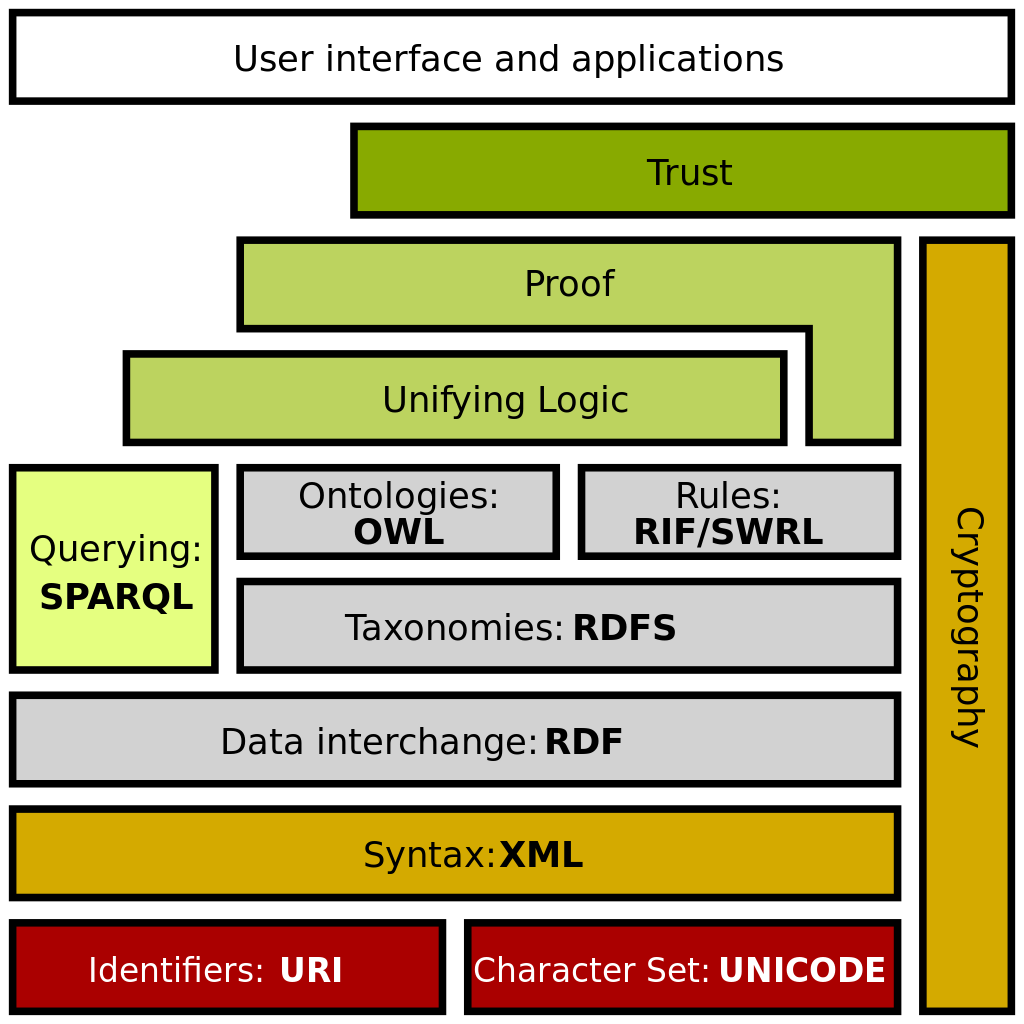
\includegraphics[width=0.6\linewidth]{semantic_web_stack}
    \caption{Arquitectura de la web semántica.} Fuente: FIXME
    \label{fig:semantic-web-arq}
\end{figure}

\subsubsection{Referencias, transporte y principios de los datos enlazados}

El acceso a los datos es fundamental para la arquitectura de la web semántica.
Podemos tomar como referencia, el modelo utilizado por los servidores
\textit{Web}, en el cual, los documentos disponibles se encuentran enlazados a
otros de forma descentralizada, esto es, que el documento referenciado no
necesariamente se encuentra en el mismo servidor que está haciendo referencia a
él. Estos enlaces, son utilizados por los usuarios para navegar entre los
millones de servidores disponibles en la \textit{Web}.

Las URI/IRI y el protocolo HTTP son parte fundamental del núcleo que define
tanto a la \textit{World Wide Web} como a la web semántica. En un ejemplo
concreto, la URI \url{https://en.wikipedia.org/wiki/Back_to_the_Future} en la
\textit{Web}, representa el documento en el servidor
\url{https://www.wikipedia.org} que contiene información sobre la serie de
películas y obras de título ``Volver al Futuro'', en cambio, en el contexto de
la web semántica, la URI \url{https://www.wikidata.org/wiki/Q1} representa al
``universo'' como una entidad, la cual es parte del
\url{https://www.wikidata.org/wiki/Q3327819} ``multiverso'' y es estudiado por
la \url{https://www.wikidata.org/wiki/Q338} ``cosmología''.

Los datos del ejemplo anterior son publicados por ``The Wikipedia Fundation" a
través del servicio Wikidata \cite{vrandevcic2014wikidata}, pero las relaciones
descritas podrían enlazar a otros editores de contenido, como por ejemplo
DBpedia \cite{valsecchi2015dbpedia}, el cual es un esfuerzo comunitario para
extraer información estructurada desde distintas fuentes y enlazarlas a través
del formato \textit{RDF}. Para lograr esto, los editores de contenido para la
web semántica aplican los siguientes principios a sus datos, los cuales son
conocidos como los ``principios para datos enlazados'' o \textit{LinkedData
principles} \cite{bizer2011linked}.

\begin{enumerate}
    \item Utilizar URIs como nombres para entidades.
    \item Utilizar URIs HTTP para que los usuarios puedan buscar y acceder a
    estas entidades.
    \item Cuando un usuario consulta una URI, debes entregar información
    relevante, utilizando estándares como \textit{RDF} y \textit{SPARQL}.
    \item Debes incluir enlaces a otras URIs, para que los usuarios descubran
    más entidades.
\end{enumerate}

\subsubsection{Intercambio de datos}
\label{sec:intercambio-datos}

\begin{figure}
    \centering
    \includesvg[width=\linewidth]{rdf-graph.svg}
    \caption{Un grafo \textit{RDF} básico.} Los nodos \textit{Subject} y
    \textit{Object} están conectados a través de la relación \textit{Predicate}.
    Fuente: FIXME.
    \label{fig:rdf-graph1}
\end{figure}

Los datos de la web semántica son generados por distintas entidades al rededor
del mundo, las cuales no están necesariamente coordinados entre ellos, por lo
que la arquitectura debe soportar la creación distribuida de datos junto con la
integración de múltiples fuentes y la interoperabilidad entre los datos creados
\cite{bizer2011linked}. Este tipo de requerimientos los cumplen las estructuras
de datos basados en grafos como \textit{RDF}. \textit{RDF} es un formato basado
en la descripción de grafos dirigidos, los cuales representan la información de
la forma de tríos sujeto - predicado - objeto, en la cual, el sujeto y el
predicado corresponden a nodos del grafo y el predicado es un arco que los
relaciona como se puede observar en la figura \ref{fig:rdf-graph1}. En estos
tríos, cualquiera de estos objetos puede tomar el valor de una URI, un valor
literal (cadenas de texto, números o fechas) o simplemente un nodo vacío
(identificadores que no pueden ser referenciados por otra entidad).

\textit{RDF} corresponde a la especificación de un lenguaje abstracto para
describir relaciones entre entidades, el cual, puede ser serializado en
múltiples formatos de texto como \textit{Extensible Markup Language (XML)}
\cite{beckett2004rdf} en la figura \ref{fig:rdf-xml-ex} o en un formato más
compacto como \textit{Turtle} \cite{beckett2014rdf} en la figura
\ref{fig:rdf-turtle-ex}.

\begin{figure}
    \centering
    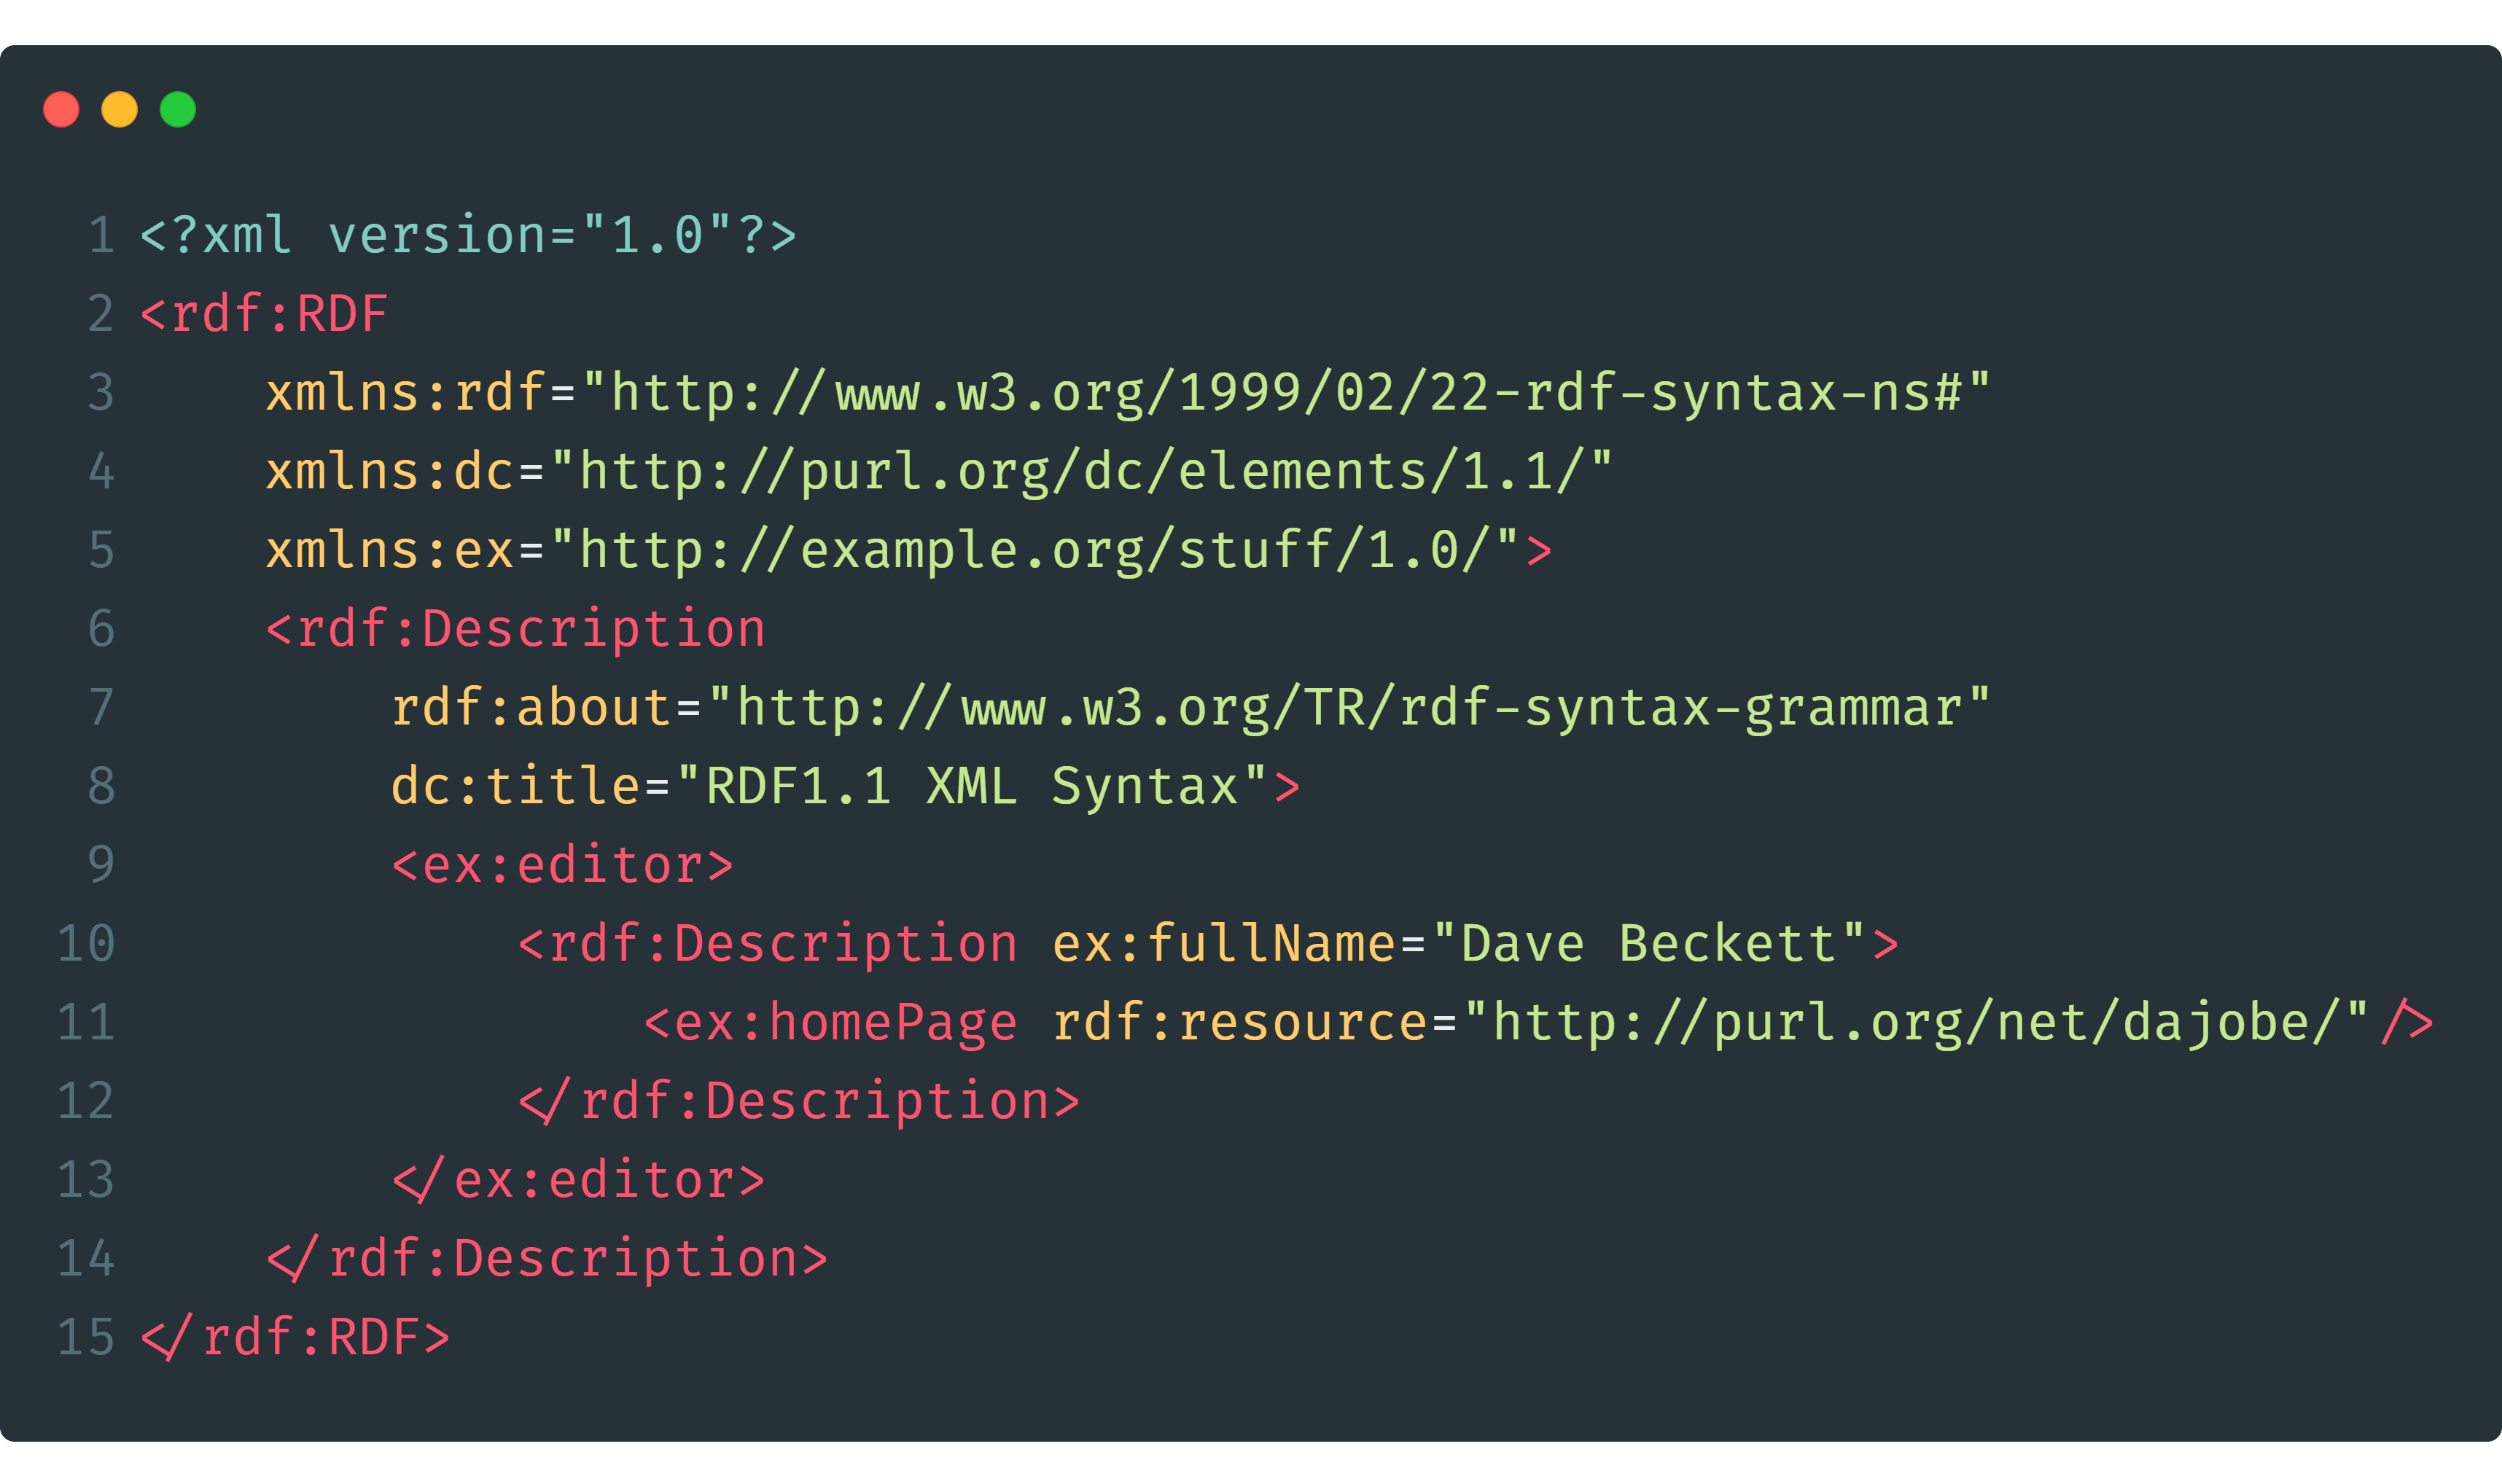
\includegraphics[width=\linewidth]{rdf-xml-ex.png}
    \caption{Descripción de un documento \textit{RDF/XML}.} Fuente: RDF 1.1 XML
    Syntax. World Wide Web Consortium.
    \label{fig:rdf-xml-ex}
\end{figure}

\begin{figure}
    \centering
    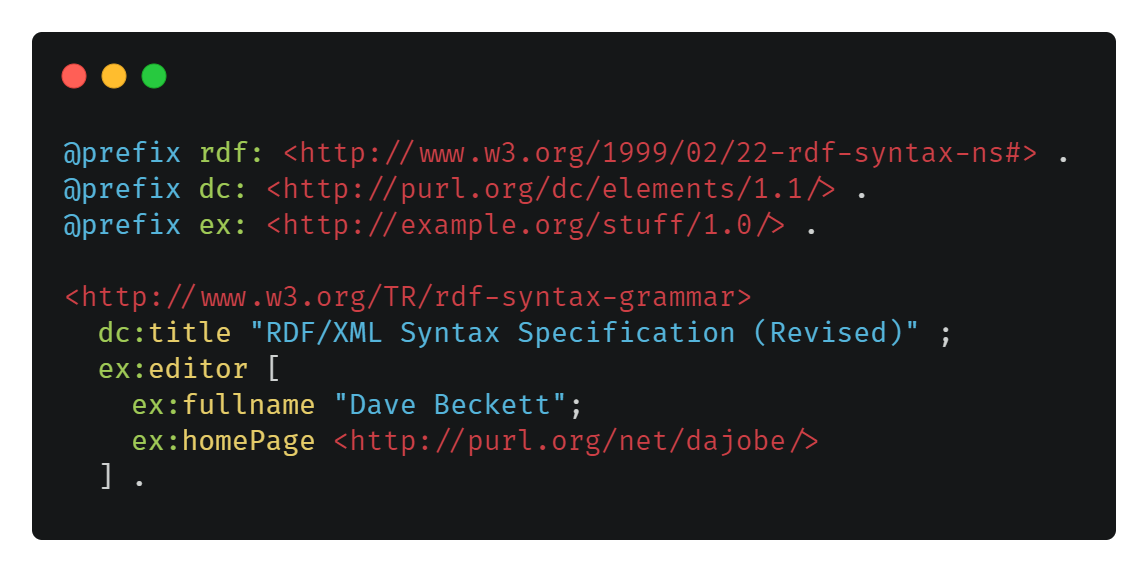
\includegraphics[width=\linewidth]{rdf-turtle-ex.png}
    \caption{Descripción de un documento \textit{RDF/Turtle}.} Fuente: Turtle
    (Syntax). Wikipedia.
    \label{fig:rdf-turtle-ex}
\end{figure}

\subsubsection{Consultas y actualizaciones}

Los principios de los datos enlazados explicados en la sección
\ref{sec:intercambio-datos} nos entregan guias sobre como realizar la
publicación y permitir el acceso a datos simples, sin embargo, no es posible
realizar consultas complejas a aquellos datos publicados utilizando estos
principios, puesto que, no es necesario contar con un sistema o mecanismo de
consulta para publicar información. Si continuamos con el ejemplo de las
peliculas ``Volver al Futuro'', consideremos que buscamos obtener los titulos de
aquellas peliculas en las que los miembros del elenco de ``Volver al Futuro''
también han actuado. Una forma relativamente sencilla de lograr esto, es acceder
a la URI que representa la pelicula, obtener las URIs de los actores y de forma
iterativa acceder a estas URIs para obtener el nombre de las peliculas en las
que cada miembro ha participado. No es dificil darse cuenta, que este proceso no
es para nada eficiente en tiempo de ejecución ni recursos de red utilizados.

Para resolver esta consulta, utilizamos el lenguaje de consultas para
repositorios \textit{RDF} llamado \textit{SPARQL}, cuyo nombre corresponde al
acronimo recursivo ``\textit{\textbf{S}PARQL \textbf{P}rotocol \textbf{A}nd
\textbf{R}DF \textbf{Q}uery \textbf{L}anguage}'' \cite{world2013sparql}. Este
lenguaje esta diseñado para evaluar consultas hacia repositorios de datos
almacenados en formato \textit{RDF}, en estos repositorios, la información no se
obtiene accediendo de forma iterativa a distintas URIs que representan
entidades, si no que enviando consultas a un \textit{endpoint} que soporta
\textit{SPARQL}. \textit{SPARQL} permite a sus usuarios especificar URIs
arbitrarias, las cuales podrian no ser accesibles a través de la \textit{Web},
junto con un patron de grafo dirigido el cual debe coincidir con los datos
disponibles en el repositorio y en el que pueden ser descritas determinadas
restricciones para los datos obtenidos. En la figura \ref{fig:graph-pattern-ex}
se puede apreciar el patron del grafo utilizado para consultar por las peliculas
en las que el elenco de ``Volver al futuro'' ha participado.

\begin{figure}
    \centering
    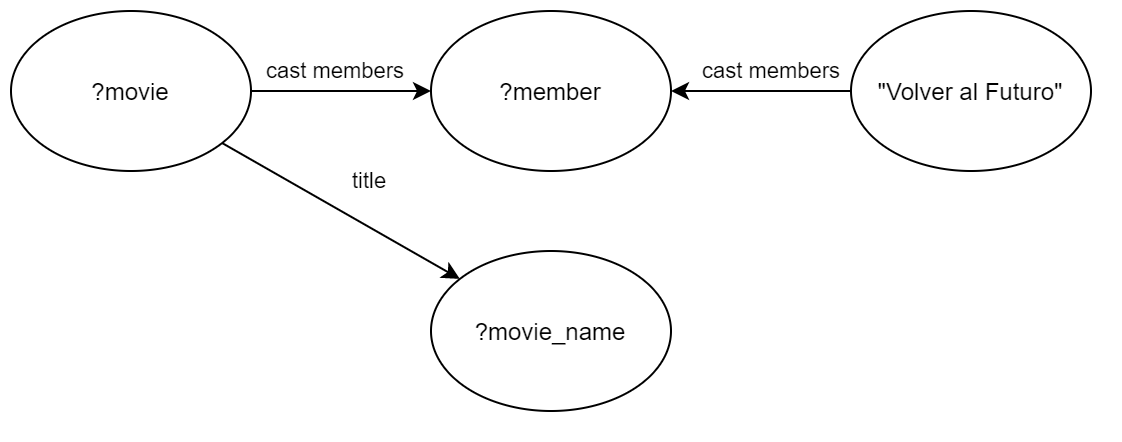
\includegraphics[width=\linewidth]{graph-pattern-ex.png}
    \caption{FIXME}
    \label{fig:graph-pattern-ex}
\end{figure}

Esta consulta puede ser representada utilizando \textit{SPARQL}, como se puede
apreciar en la figura \ref{fig:graph-pattern-ex-sparql}. Una consulta
\textit{SPARQL} esta compuesta de multiples secciones, las sentencias
\textit{\texttt{PREFIX}} son utilizadas para abreviar URIs y su rol es apoyar la
legibilidad de la consulta. El nucleo de una consulta se encuentra en la sección
\textit{\texttt{WHERE}}, en la cual, se debe definir de forma precisa el patrón
de nuestro grafo dirigido, el cual debe coincidir con la información semántica
disponible. Un patrón básico consiste de patrones individuales los cuales pueden
ser sujetos, predicados u objetos unidos por variables, formando una plantilla,
la cual será completada en el proceso de evaluación de la consulta. De forma
opcional, una sentencia \textit{\texttt{WHERE}} puede estar acompañada de una
expresión \textit{\texttt{FILTER}} la cual puede acotar los resultados obtenidos
a determinadas estrucutras que cumplan con creiterios especificados.

\begin{figure}
    \centering
    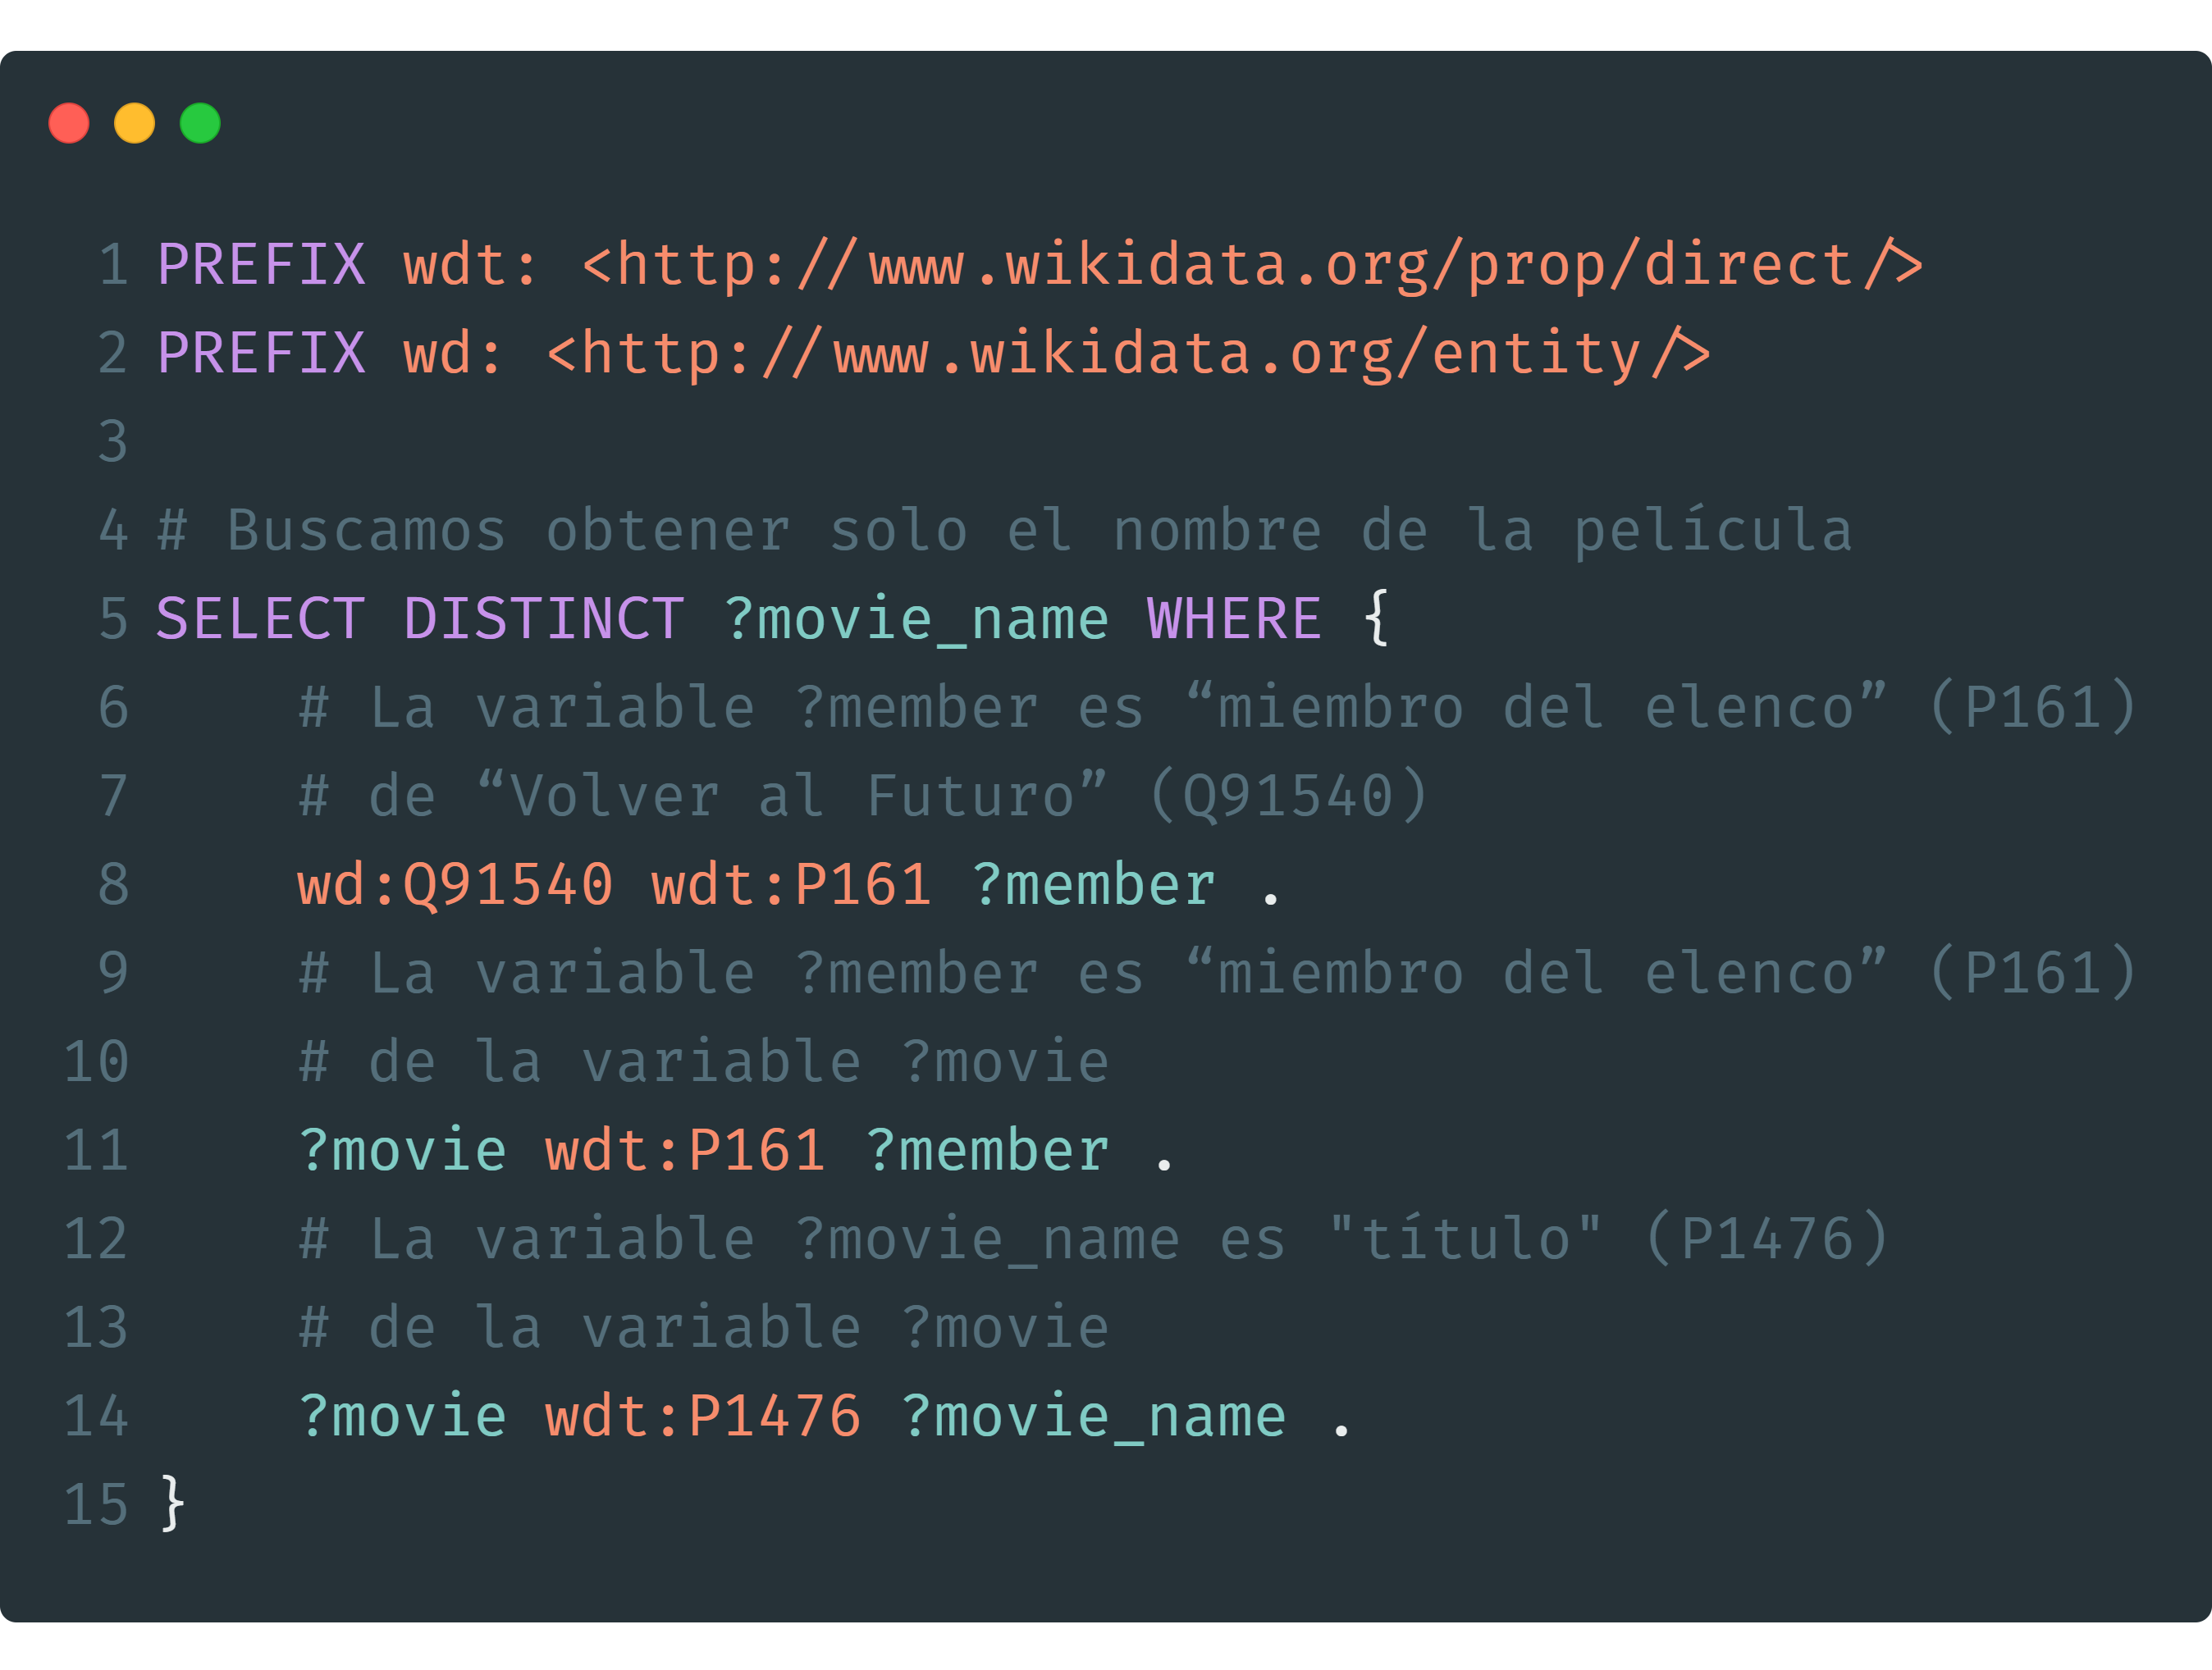
\includegraphics[width=0.85\linewidth]{graph-pattern-ex-sparql.png}
    \caption{FIXME}
    \label{fig:graph-pattern-ex-sparql}
\end{figure}

FIXME: REFS FIXME: Updated ranking of implementations

La especificación \textit{SPARQL} puede ser implementada en multiples
repositorios orientados a grafos, entre los populares se encuentran Sesame 16,
Jena 52, Virtuoso 77, BigData 9, OWLIM 60 y RDF-3X 55. Debido a que en muchas
ocaciones los datos estan almacenados en bases de datos relacionales, se
necesitan \textit{wrappers} que nos permitan acceder a estos datos a través de
\textit{APIs}. Ejemplos conocidos de estos \textit{wrappers} son DR2 10 y
Triplify 13. Estas herramientas permiten que fuentes de datos legadas puedan ser
expuestas y consultadas como grafos semánticos, lo cual facilita la transición
hacia estas nuevas técnologias.

Además de la especificación de un lenguaje, \textit{SPARQL} define los
protocolos de acceso y formatos interoperables para los conjuntos de datos
almacenados. Los datos son expuestos a través de HTTP lo cual permite un libre
acceso y elimina la necesidad de los usuarios de descargar estos datos para
consultarlos.

Actualmente el estándar \textit{SPARQL} permite realizar consultas a una unica
fuente de datos a la vez. Para acceder a datos de multiples fuentes al mismo
tiempo es posible realizar multiples consultas secuenciales a los distintos
repositorios, sin embargo, la responsabilidad de unir estos resultados de forma
consistente pasa a ser del usuario que realiza la consulta. Actualmente se esta
diseñando una solución alternativa para realizar consultas federadas. [FIXME:
ESTO PARECE DESACTUALIZADO, BUSCAR UNA MEJOR FUENTE]

\subsubsection{Ontologías y razonamiento}

Para codificar un significado a nuestros datos debemos utilizar construcciones
logicas. Las técnologias que habilitan el razonamiento para la \textit{web}
semántica son los esquemas \textit{RDF}, el lenguaje de
ontologías\footnote{Definir una ontología} \textit{OWL (Web Ontology Language)}
\cite{antoniou2004web} y \textit{RIF (Rule Interchange Format)}
\cite{kifer2008rule}.

Para explicar el razonamiento en la \textit{web} semántica, esto es, generar
conclusiones en base a hechos y verdades disponibles en nuestros repositorios de
datos, podemos utilizar un conjunto de ontologías aplicado al ejemplo que hemos
utilizado en las secciones anteriores a través de las propiedades
\texttt{rdfs:subClassOf} y \texttt{owl:sameAs}. La propiedad
\texttt{rdfs:subClassOf} puede ser utilizada para definir jerarquias de clases.
Consideremos el siguiente ejemplo, definiremos una ontología llamada
\texttt{OntologíaFormula1} en el contexto de la competencia de automovilismo
internacional, esta ontología define dos clases: \texttt{f1:Competidores},
\texttt{f1:Equipo} y contiene un axioma\footnote{Definir axioma} el cual indica
que \texttt{f1:Equipo} es una subclase de \texttt{f1:Competidores} a través de
la propiedad \texttt{rdfs:subClassOf}. Esta relación le permite a un agente
inteligente deducir que las instancias de \texttt{f1:Equipo} también son del
tipo \texttt{f1:Competidores}, de esta forma si en nuetro repositorio existen
los registros ``Charles Leclerc'' del tipo \texttt{f1:Competidores} y
``Ferrari'' del tipo \texttt{f1:Equipo}, cuando realizemos una consulta por
todas las entidades del tipo \texttt{f1:Competidores} obtendremos como resultado
``Charles Leclerc'' y ``Ferrari'' incluso cuando las instancias no especifican
esta relación de forma explicita.

Otra propiedades importante es \texttt{owl:sameAs}, la cual puede ser usada para
especificar que dos recursos son identicos, incluso cuando se encuentran en
repositorios distintos. Por ejemplo, podemos indicar que el recurso
\url{https://www.wikidata.org/wiki/Q27586} es identico a
\url{http://dbpedia.org/page/Ferrari}, lo que permite a nuestro agente inteligente consolidar
información más completa para una entidad determinada desde multiples fuentes de
datos.

\subsubsection{Reglas}

Otro mecanismo que nos permite generar conclusiones en base a datos existentes
son las regals logicas. Estas reglas estan compuestas de dos secciones,
antecedentes y consequencias: si se cumplen las sentencias en los antecedentes,
entonces las sentencias de la consequencias son verdaderas. La \textit{W3C}
recomienda utilizar \textit{RIF} ?? para intercambiar reglas entre sistemas. El
conjunto común de reglas utilizadas en multiples sistemas ha sido estandarizado
en \textit{RIF Core} 12.

\subsubsection{Seguridad y encriptación}

En un sistema global abierto como la \textit{Internet}, donde la información es
transmitida a través de canales inseguros y sin autenticación utilizando
infraestrucutura mantenida por una gran cantidad de organizaciones es necesario
definir mecanismos y protocolos para realizar intercambios de información de
forma segura. Estos problemas son abordados utilizando la capa de criptografia
en la \textit{web} semántica.

Para asegurar que los datos no son alterados durante su transmisión se utiliza
el protocolo HTTPS 66 el cual implementa encriptación para proteger la
información de ataques \textit{man-in-the-middle}\footnote{Explicar MITM}.

El estandar \textit{RDF} utiliza firmas digitales para asegurar la autenticidad
del contenido entregado por los repositorios de datos. Este proceso se realiza
utilizando metodos estandar y conocidos de firma electronica 17, lo que permite
demostrar que el contenido proviene de una fuente confiable y que no ha sido
modificado.

Si buscamos establecer la identidad de un usuario que intenta utilizar un
servicio determinado podemos utilizar sistemas como OpenID 57, en el cual, los
usuarios son redirigidos a un portal donde se verifican sus credenciales y se
obtiene su identidad digital. [FIXME: MÁS TECNICAS DE AUTENTICACIÓN]

\subsubsection{Unificación e integración}

El proceso de unificación 

\subsubsection{Confianza}

\subsubsection{Aplicaciones}

\subsection{Generación de sugerencias}

\subsubsection{Indexación de documentos}

\subsubsection{Ranking de resultados}

\subsection{RDFExplorer}

